\documentclass[tikz,border=12pt]{standalone}
\usepackage[T1]{fontenc}
\usepackage{mathpazo}
\usepackage{amsmath,amssymb}
\usetikzlibrary{arrows.meta, positioning, calc, fit, decorations.pathreplacing}
\definecolor{stblue}{HTML}{7B97AD}
\definecolor{rwgold}{HTML}{B8995E}
\definecolor{sage}{HTML}{7A9A7E}
\definecolor{dkbrown}{HTML}{3D3530}
\definecolor{wmgray}{HTML}{7B7067}
\definecolor{cream}{HTML}{F9F6F0}
\definecolor{border}{HTML}{D4C9B8}
\definecolor{terracotta}{HTML}{C47A6A}
\definecolor{lavender}{HTML}{907EA0}

\begin{document}
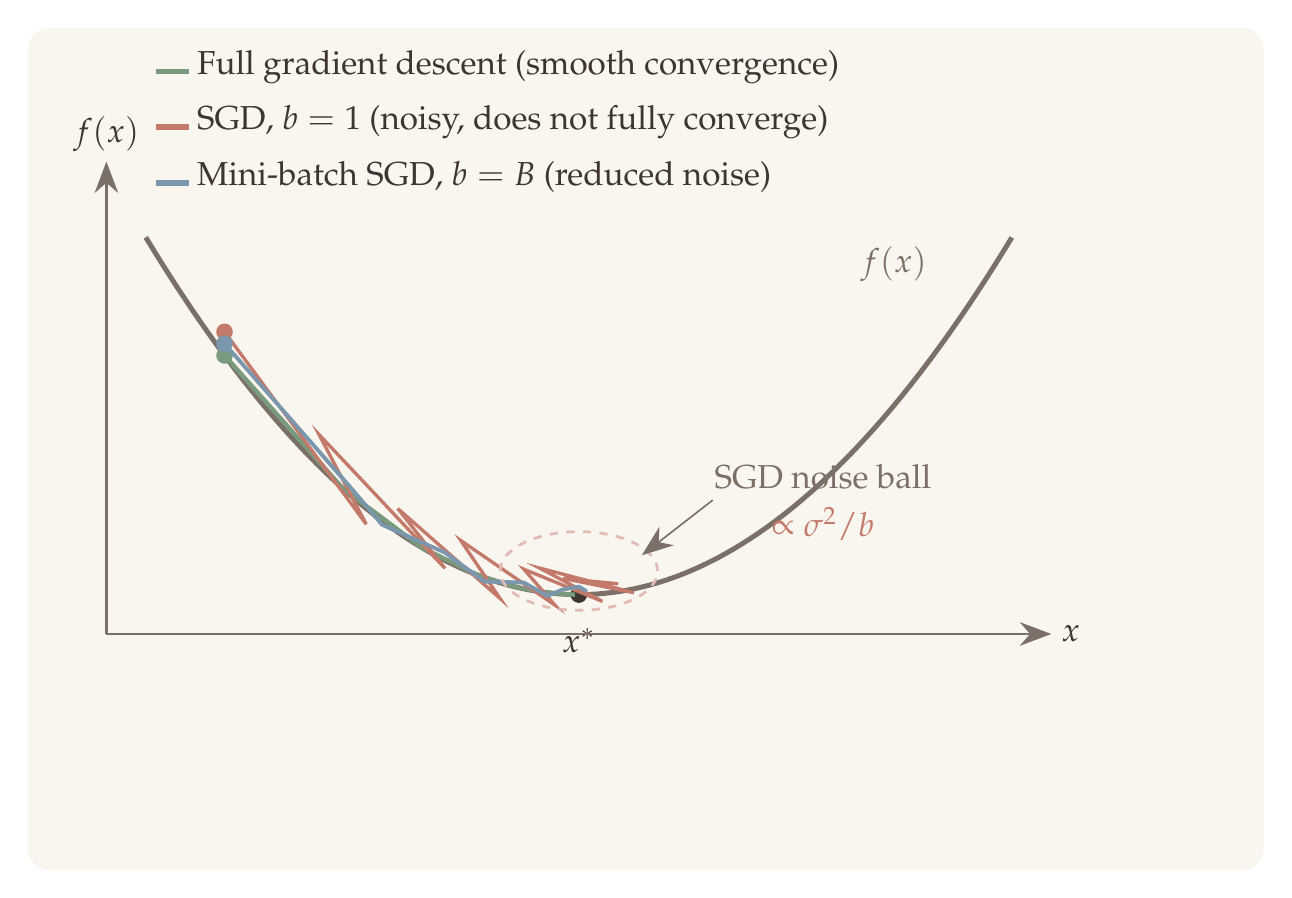
\begin{tikzpicture}[
    >={Stealth[length=4mm, width=3mm]},
    every node/.style={text=dkbrown},
  ]

  % Background
  \fill[cream, rounded corners=8pt] (-1.5,-2.5) rectangle (14.2,8.2);

  % === Objective function (smooth convex curve) ===
  % f(x) = 0.15*(x-5.5)^2 + 1
  \draw[wmgray, line width=1.8pt, smooth, domain=0:11, samples=100]
    plot (\x, {0.15*(\x-5.5)*(\x-5.5) + 1.0});

  % Optimal point
  \fill[dkbrown] (5.5, 1.0) circle (3pt);
  \node[font=\large\bfseries, below] at (5.5, 0.7) {$x^*$};

  % Axes
  \draw[->, wmgray, line width=0.8pt] (-0.5, 0.5) -- (11.5, 0.5)
    node[right, font=\large] {$x$};
  \draw[->, wmgray, line width=0.8pt] (-0.5, 0.5) -- (-0.5, 6.5)
    node[above, font=\large] {$f(x)$};

  % === Full GD trajectory (smooth) ===
  \draw[sage, line width=1.6pt, smooth]
    (1.0, {0.15*(1.0-5.5)*(1.0-5.5)+1.0})
    -- (2.5, {0.15*(2.5-5.5)*(2.5-5.5)+1.0})
    -- (3.5, {0.15*(3.5-5.5)*(3.5-5.5)+1.0})
    -- (4.2, {0.15*(4.2-5.5)*(4.2-5.5)+1.0})
    -- (4.7, {0.15*(4.7-5.5)*(4.7-5.5)+1.0})
    -- (5.0, {0.15*(5.0-5.5)*(5.0-5.5)+1.0})
    -- (5.2, {0.15*(5.2-5.5)*(5.2-5.5)+1.0})
    -- (5.35, {0.15*(5.35-5.5)*(5.35-5.5)+1.0})
    -- (5.45, {0.15*(5.45-5.5)*(5.45-5.5)+1.0});
  \fill[sage] (1.0, {0.15*(1.0-5.5)*(1.0-5.5)+1.0}) circle (3pt);

  % === SGD trajectory (noisy zigzag) ===
  \draw[terracotta, line width=1.2pt]
    (1.0, {0.15*(1.0-5.5)*(1.0-5.5)+1.0+0.3})
    -- (2.8, {0.15*(2.8-5.5)*(2.8-5.5)+1.0-0.2})
    -- (2.2, {0.15*(2.2-5.5)*(2.2-5.5)+1.0+0.4})
    -- (3.8, {0.15*(3.8-5.5)*(3.8-5.5)+1.0-0.1})
    -- (3.2, {0.15*(3.2-5.5)*(3.2-5.5)+1.0+0.3})
    -- (4.5, {0.15*(4.5-5.5)*(4.5-5.5)+1.0-0.2})
    -- (4.0, {0.15*(4.0-5.5)*(4.0-5.5)+1.0+0.35})
    -- (5.2, {0.15*(5.2-5.5)*(5.2-5.5)+1.0-0.15})
    -- (4.8, {0.15*(4.8-5.5)*(4.8-5.5)+1.0+0.25})
    -- (5.8, {0.15*(5.8-5.5)*(5.8-5.5)+1.0-0.1})
    -- (5.0, {0.15*(5.0-5.5)*(5.0-5.5)+1.0+0.3})
    -- (6.2, {0.15*(6.2-5.5)*(6.2-5.5)+1.0-0.05})
    -- (5.3, {0.15*(5.3-5.5)*(5.3-5.5)+1.0+0.2})
    -- (6.0, {0.15*(6.0-5.5)*(6.0-5.5)+1.0+0.1});
  \fill[terracotta] (1.0, {0.15*(1.0-5.5)*(1.0-5.5)+1.0+0.3}) circle (3pt);

  % === Mini-batch SGD trajectory (mildly noisy) ===
  \draw[stblue, line width=1.4pt]
    (1.0, {0.15*(1.0-5.5)*(1.0-5.5)+1.0+0.15})
    -- (2.6, {0.15*(2.6-5.5)*(2.6-5.5)+1.0+0.1})
    -- (3.0, {0.15*(3.0-5.5)*(3.0-5.5)+1.0-0.05})
    -- (3.8, {0.15*(3.8-5.5)*(3.8-5.5)+1.0+0.1})
    -- (4.3, {0.15*(4.3-5.5)*(4.3-5.5)+1.0-0.05})
    -- (4.8, {0.15*(4.8-5.5)*(4.8-5.5)+1.0+0.08})
    -- (5.1, {0.15*(5.1-5.5)*(5.1-5.5)+1.0-0.04})
    -- (5.3, {0.15*(5.3-5.5)*(5.3-5.5)+1.0+0.06})
    -- (5.5, {0.15*(5.5-5.5)*(5.5-5.5)+1.0+0.1})
    -- (5.6, {0.15*(5.6-5.5)*(5.6-5.5)+1.0+0.04});
  \fill[stblue] (1.0, {0.15*(1.0-5.5)*(1.0-5.5)+1.0+0.15}) circle (3pt);

  % === Noise ball around optimum ===
  \draw[terracotta!50, line width=1pt, dashed] (5.5, 1.3) ellipse (1.0cm and 0.5cm);
  \draw[->, wmgray, line width=0.6pt] (7.2, 2.2) -- (6.3, 1.5);
  \node[font=\large, wmgray, align=center] at (8.6, 2.5)
    {SGD noise ball};
  \node[font=\large, terracotta, align=center] at (8.6, 1.9)
    {$\propto \sigma^2 / b$};

  % === Legend ===
  \node[font=\large, anchor=west] at (0.0, 7.7)
    {\textcolor{sage}{\rule{12pt}{2pt}} Full gradient descent (smooth convergence)};
  \node[font=\large, anchor=west] at (0.0, 7.0)
    {\textcolor{terracotta}{\rule{12pt}{2pt}} SGD, $b = 1$ (noisy, does not fully converge)};
  \node[font=\large, anchor=west] at (0.0, 6.3)
    {\textcolor{stblue}{\rule{12pt}{2pt}} Mini-batch SGD, $b = B$ (reduced noise)};

  % === Objective label ===
  \node[font=\large, wmgray] at (9.5, 5.2) {$f(x)$};

\end{tikzpicture}
\end{document}
